\documentclass[12pt,a4paper]{article}
\usepackage{fontspec}
\usepackage[polish]{babel}
\usepackage[a4paper,margin=2.5cm]{geometry}
\usepackage{setspace}
\setstretch{1.3}
\usepackage{graphicx}
\usepackage{booktabs}
\usepackage{tabularx}
\usepackage{amsmath}
\usepackage{float}
\usepackage{caption}
\usepackage{subcaption}
\usepackage{xcolor}
\usepackage{listings}
\usepackage{enumitem}
\usepackage[hidelinks]{hyperref}
\usepackage{xurl}

\graphicspath{{img/}}
\setlength{\emergencystretch}{3em}
\captionsetup{labelsep=colon,font={small,stretch=1}}
\captionsetup[table]{position=top}

\lstset{
  language=Python,
  basicstyle=\ttfamily\footnotesize\setstretch{1},
  keywordstyle=\color{teal!70!black},
  commentstyle=\color{black!55}\itshape,
  stringstyle=\color{red!65!black},
  showstringspaces=false,
  breaklines=true,
  frame=single,
  rulecolor=\color{black},
  framesep=4pt,
  xleftmargin=4pt,
  xrightmargin=4pt,
  aboveskip=6pt,
  belowskip=10pt,
}

\newcommand{\przedmiot}{Urządzenia peryferyjne}
\newcommand{\termin}{poniedziałek 23.11.2026 grupa 8.00}
\newcommand{\temat}{Kamery cyfrowe}

\newcommand{\stronatytulowa}[1]{%
  \begin{titlepage}
    \centering
    \vspace*{1.2cm}
    \colorbox{black!4}{\parbox{3.6cm}{\centering\vspace{6pt}%
      
\includegraphics[width=2.9cm]{pwr_logo_bw.png}\\[4pt]
      {\sffamily\large\setstretch{1}Politechnika\\Wrocławska\par}\vspace{6pt}}}\par
    \vspace{2.8cm}
    {\large\textsc{\przedmiot}\par}
    \vspace{0.5cm}
    {\textsc{\termin}\par}
    \vspace{1.2cm}
    \rule{\linewidth}{1pt}\par
    \vspace{0.5cm}
    {\LARGE\bfseries\setstretch{1}\temat\\#1\par}
    \vspace{0.4cm}
    \rule{\linewidth}{1pt}\par
    \vspace{0.6cm}
    \begin{minipage}[t]{0.48\textwidth}
      \raggedright\setstretch{1.25}
      \emph{Autorzy:}\\
      Iga \textsc{Wolanin} 281203\\
      Adam \textsc{Korwin} 284455
    \end{minipage}\hfill
    \begin{minipage}[t]{0.48\textwidth}
      \raggedleft\setstretch{1.25}
      \vspace{0.3cm}
      \emph{Prowadzący:}\\
      dr inż. Dominik \textsc{Żelazny}
    \end{minipage}
    \vfill
  \end{titlepage}
}


\begin{document}
\stronatytulowa{Raport}

\section{Przebieg ćwiczenia}
Celem ćwiczenia było napisanie programu, który wykrywa kamery podłączone do komputera, pozwala
wybrać kamerę i jakość obrazu (rozdzielczość), zmieniać nasycenie i inne parametry obrazu, a także
wykonuje zdjęcia i nagrywa filmy. Ćwiczenie wykonano na komputerze MacBook Air z systemem macOS,
do którego przez przejściówkę USB-C podłączono dwie kamery USB: Microsoft LifeCam HD-3000 oraz
kamerę Megapixel (w systemie widoczną jako \texttt{USB2.0 Camera}). Program napisano w Pythonie z użyciem bibliotek OpenCV (odczyt klatek,
przetwarzanie obrazu, zapis plików), tkinter (interfejs graficzny) oraz PyObjC z modułami
AVFoundation i CoreMedia (nazwy kamer i formaty pracy sensora w systemie macOS).

\textbf{Na ocenę wyższą zrealizowano zadanie 2 w wariancie wykrywania ruchu.} Program
\texttt{ruch\_mac.py} zawiera wszystkie funkcje zadania 1 oraz dodatkowy panel wykrywania ruchu:
obrysowanie poruszających się obiektów i automatyczne zdjęcie przy wykryciu ruchu.

\section{Opis programu}
Program składa się z trzech plików. Plik \texttt{kamera.py} zawiera klasę \texttt{App} z całą
obsługą kamery, parametrów obrazu i zapisu (zadanie 1). Plik \texttt{macos/kamera\_mac.py} zawiera
klasę \texttt{MacApp}, która dziedziczy po \texttt{App} i zastępuje wykrywanie kamer oraz zmianę
rozdzielczości wersjami korzystającymi z AVFoundation. Plik \texttt{macos/ruch/ruch\_mac.py}
łączy \texttt{MacApp} z klasą \texttt{MotionApp} (wykrywanie ruchu, ocena wyższa).
Program uruchamia się skryptem \texttt{./macos/ruch/start.sh}, który przy pierwszym uruchomieniu
tworzy środowisko \texttt{.venv} i instaluje biblioteki. Zdjęcia i filmy trafiają do folderu
\texttt{nagrania/}. Poniżej opisano najważniejsze części programu. Pominięto importy i budowę
interfejsu, a wielokropek (\texttt{...}) oznacza pominięty kod.

\subsection{Wykrywanie kamer i dostęp do kamery}
Przed użyciem kamery macOS wymaga zgody użytkownika. Stan zgody sprawdza funkcja
\texttt{ensure\_camera\_access()}, która w razie potrzeby wyświetla systemowe zapytanie. Funkcja
\texttt{av\_devices()} pobiera listę kamer z AVFoundation. Lista jest sortowana po
identyfikatorze \texttt{uniqueID}, ponieważ w tej samej kolejności OpenCV numeruje kamery.
Dzięki temu nazwa na liście (np. kamera USB lub wbudowana kamera MacBooka) odpowiada
indeksowi przekazywanemu do \texttt{cv2.VideoCapture}.
\begin{lstlisting}
def av_devices():
    devs = list(AVF.AVCaptureDevice.devicesWithMediaType_(AVF.AVMediaTypeVideo)) + \
        list(AVF.AVCaptureDevice.devicesWithMediaType_(AVF.AVMediaTypeMuxed))
    return sorted(devs, key=lambda d: d.uniqueID())

class MacApp(App):
    def detect_cameras(self):
        ...
        if ensure_camera_access(self.root):
            self.devices = av_devices()
        self.cameras = [(i, d.localizedName()) for i, d in enumerate(self.devices)]
\end{lstlisting}

\subsection{Połączenie i rozdzielczość}
Po wybraniu kamery i przycisku \emph{Połącz} program otwiera kamerę przez
\texttt{cv2.VideoCapture} i uruchamia osobny wątek, który odczytuje klatki. Odczyt w wątku
interfejsu blokowałby okno programu.
\begin{lstlisting}
def grab_loop(self, cap):
    while self.cap is cap:
        with self.cap_lock:
            ok, frame = cap.read()
        if ok and frame is not None:
            self.latest = frame
            self.seq += 1
\end{lstlisting}
W systemie macOS samo ustawienie szerokości i wysokości klatki w OpenCV nie zmienia trybu pracy
sensora. Dlatego \texttt{apply\_resolution()} pobiera listę formatów kamery (rozmiar i maksymalna
liczba klatek na sekundę), wybiera format o żądanym rozmiarze i ustawia go jako aktywny format
urządzenia. Lista rozdzielczości w programie pokazuje tylko formaty, które kamera naprawdę obsługuje.
\begin{lstlisting}
def apply_resolution(self):
    ...
    w, h = map(int, self.res_var.get().split("x"))
    fmt = pick_format(self.formats, w, h)
    with self.cap_lock:
        if fmt:
            ok, _ = self.device.lockForConfiguration_(None)
            if ok:
                self.device.setActiveFormat_(fmt[3])
                self.device.unlockForConfiguration()
        self.cap.set(cv2.CAP_PROP_FRAME_WIDTH, w)
        self.cap.set(cv2.CAP_PROP_FRAME_HEIGHT, h)
\end{lstlisting}

\subsection{Zmiana parametrów obrazu}
Parametry obrazu zmienia się suwakami: jasność ($-100$ do $100$), kontrast (0,2 do 3,0),
nasycenie (0,0 do 3,0) i gamma (0,2 do 3,0). Dostępne są też skala szarości i odbicie lustrzane.
Funkcja \texttt{adjust()} przetwarza każdą klatkę, więc zmiany widać na podglądzie, na zdjęciach
i w nagrywanym filmie.
\begin{lstlisting}
def adjust(frame, brightness=0, contrast=1.0, saturation=1.0, gamma=1.0, gray=False, mirror=False):
    out = frame
    if contrast != 1.0 or brightness != 0:
        out = cv2.convertScaleAbs(out, alpha=contrast, beta=brightness)
    if saturation != 1.0 and not gray:
        hsv = cv2.cvtColor(out, cv2.COLOR_BGR2HSV).astype(np.float32)
        hsv[..., 1] = np.clip(hsv[..., 1] * saturation, 0, 255)
        out = cv2.cvtColor(hsv.astype(np.uint8), cv2.COLOR_HSV2BGR)
    if gamma != 1.0:
        lut = np.array([((i / 255.0) ** (1.0 / gamma)) * 255 for i in range(256)], np.uint8)
        out = cv2.LUT(out, lut)
    if gray:
        out = cv2.cvtColor(cv2.cvtColor(out, cv2.COLOR_BGR2GRAY), cv2.COLOR_GRAY2BGR)
    ...
\end{lstlisting}

\subsection{Zapis zdjęć i filmów}
Zdjęcie zapisywane jest w formacie JPG, PNG lub BMP. Dla JPG suwak ustawia jakość kompresji
(10–100\,\%). Nazwa pliku zawiera datę i godzinę z milisekundami. Film nagrywany jest jako MP4
(kodek \texttt{mp4v}) albo AVI (kodek \texttt{MJPG}). Liczba klatek na sekundę w pliku jest równa
liczbie klatek zmierzonej na podglądzie, dzięki czemu film odtwarza się z prawidłową prędkością.
\begin{lstlisting}
VIDEO_CODECS = {"mp4": "mp4v", "avi": "MJPG"}

def toggle_record(self):
    ...
    h, w = self.frame.shape[:2]
    fps = self.fps if 1 <= self.fps <= 60 else 20.0
    self.rec_path = os.path.join(OUT_DIR, f"film_{stamp()}.{ext}")
    self.writer = cv2.VideoWriter(self.rec_path, cv2.VideoWriter_fourcc(*VIDEO_CODECS[ext]),
                                  fps, (w, h))
\end{lstlisting}

\subsection{Wykrywanie ruchu (zadanie na ocenę wyższą)}
Wykrywanie ruchu zrealizowano jako zadanie dodatkowe na ocenę wyższą. Klasa
\texttt{MotionDetector} przechowuje model tła jako średnią ruchomą poprzednich klatek.
Każda nowa klatka jest zamieniana na odcienie szarości i rozmywana filtrem Gaussa, a następnie
porównywana z tłem. Piksele, które różnią się od tła o więcej niż próg, tworzą maskę ruchu.
Kontury maski o polu większym niż \emph{min. pole} obrysowywane są na podglądzie czerwonym
prostokątem. Opcja \emph{Auto-zdjęcie przy ruchu} zapisuje zdjęcie \texttt{ruch\_*.jpg},
nie częściej niż co 2 sekundy. Przycisk \emph{Zapamiętaj tło od nowa} zeruje model tła po
zmianie sceny.
\begin{lstlisting}
def detect(self, frame):
    gray = cv2.GaussianBlur(cv2.cvtColor(frame, cv2.COLOR_BGR2GRAY), (21, 21), 0)
    if self.background is None or self.background.shape != gray.shape:
        self.background = gray.astype(np.float32)
        return []
    diff = cv2.absdiff(gray, cv2.convertScaleAbs(self.background))
    cv2.accumulateWeighted(gray, self.background, self.learn_rate)
    mask = cv2.dilate(cv2.threshold(diff, self.threshold, 255, cv2.THRESH_BINARY)[1],
                      None, iterations=2)
    contours, _ = cv2.findContours(mask, cv2.RETR_EXTERNAL, cv2.CHAIN_APPROX_SIMPLE)
    return [cv2.boundingRect(c) for c in contours if cv2.contourArea(c) >= self.min_area]
\end{lstlisting}
Wersja na MacBooka łączy obie klasy przez dziedziczenie wielokrotne. \texttt{MacApp} dostarcza
obsługę kamery w macOS, a \texttt{MotionApp} dokłada panel ruchu i rysowanie prostokątów.
\begin{lstlisting}
class MacMotionApp(MacApp, MotionApp):
    TITLE = "Lab 7 - Kamera (macOS) - wykrywanie ruchu"
\end{lstlisting}
Prostokąty rysowane są tylko na kopii klatki wyświetlanej na podglądzie, więc nie trafiają do
zapisywanych zdjęć i filmów.

\section{Wyniki}
Program wykrył obie kamery USB oraz wbudowaną kamerę MacBooka i kamerę iPhone'a (Continuity
Camera). Tabela~\ref{tab:kamery} przedstawia rozdzielczości, które program odczytał z każdej kamery.
Każdą z nich ustawiono w programie i sprawdzono rozmiar odebranej klatki; we wszystkich
przypadkach był on równy wybranej rozdzielczości.

\begin{table}[H]
  \centering
  \caption{Kamery wykryte przez program i dostępne rozdzielczości}
  \label{tab:kamery}
  \begin{tabularx}{\textwidth}{lXc}
    \toprule
    Nazwa w programie & Rozdzielczości (format sensora) & Klatki/s (pomiar) \\
    \midrule
    \texttt{USB2.0 Camera} (Megapixel) & $160\times120$, $176\times144$, $320\times240$, $352\times288$, $640\times480$ & 31 \\
    \texttt{Microsoft® LifeCam HD-3000} & 13 formatów od $160\times120$ do $1280\times800$, m.in.\ $640\times480$, $1280\times720$ & 26--32 \\
    \texttt{MacBook Air Camera} & $640\times480$, $1280\times720$, $1920\times1080$ i inne & 31 \\
    \bottomrule
  \end{tabularx}
\end{table}

Rysunek~\ref{fig:okno} przedstawia okno programu z panelem kamery, suwakami parametrów obrazu,
panelem zapisu i panelem wykrywania ruchu.

\begin{figure}[H]
  \centering
  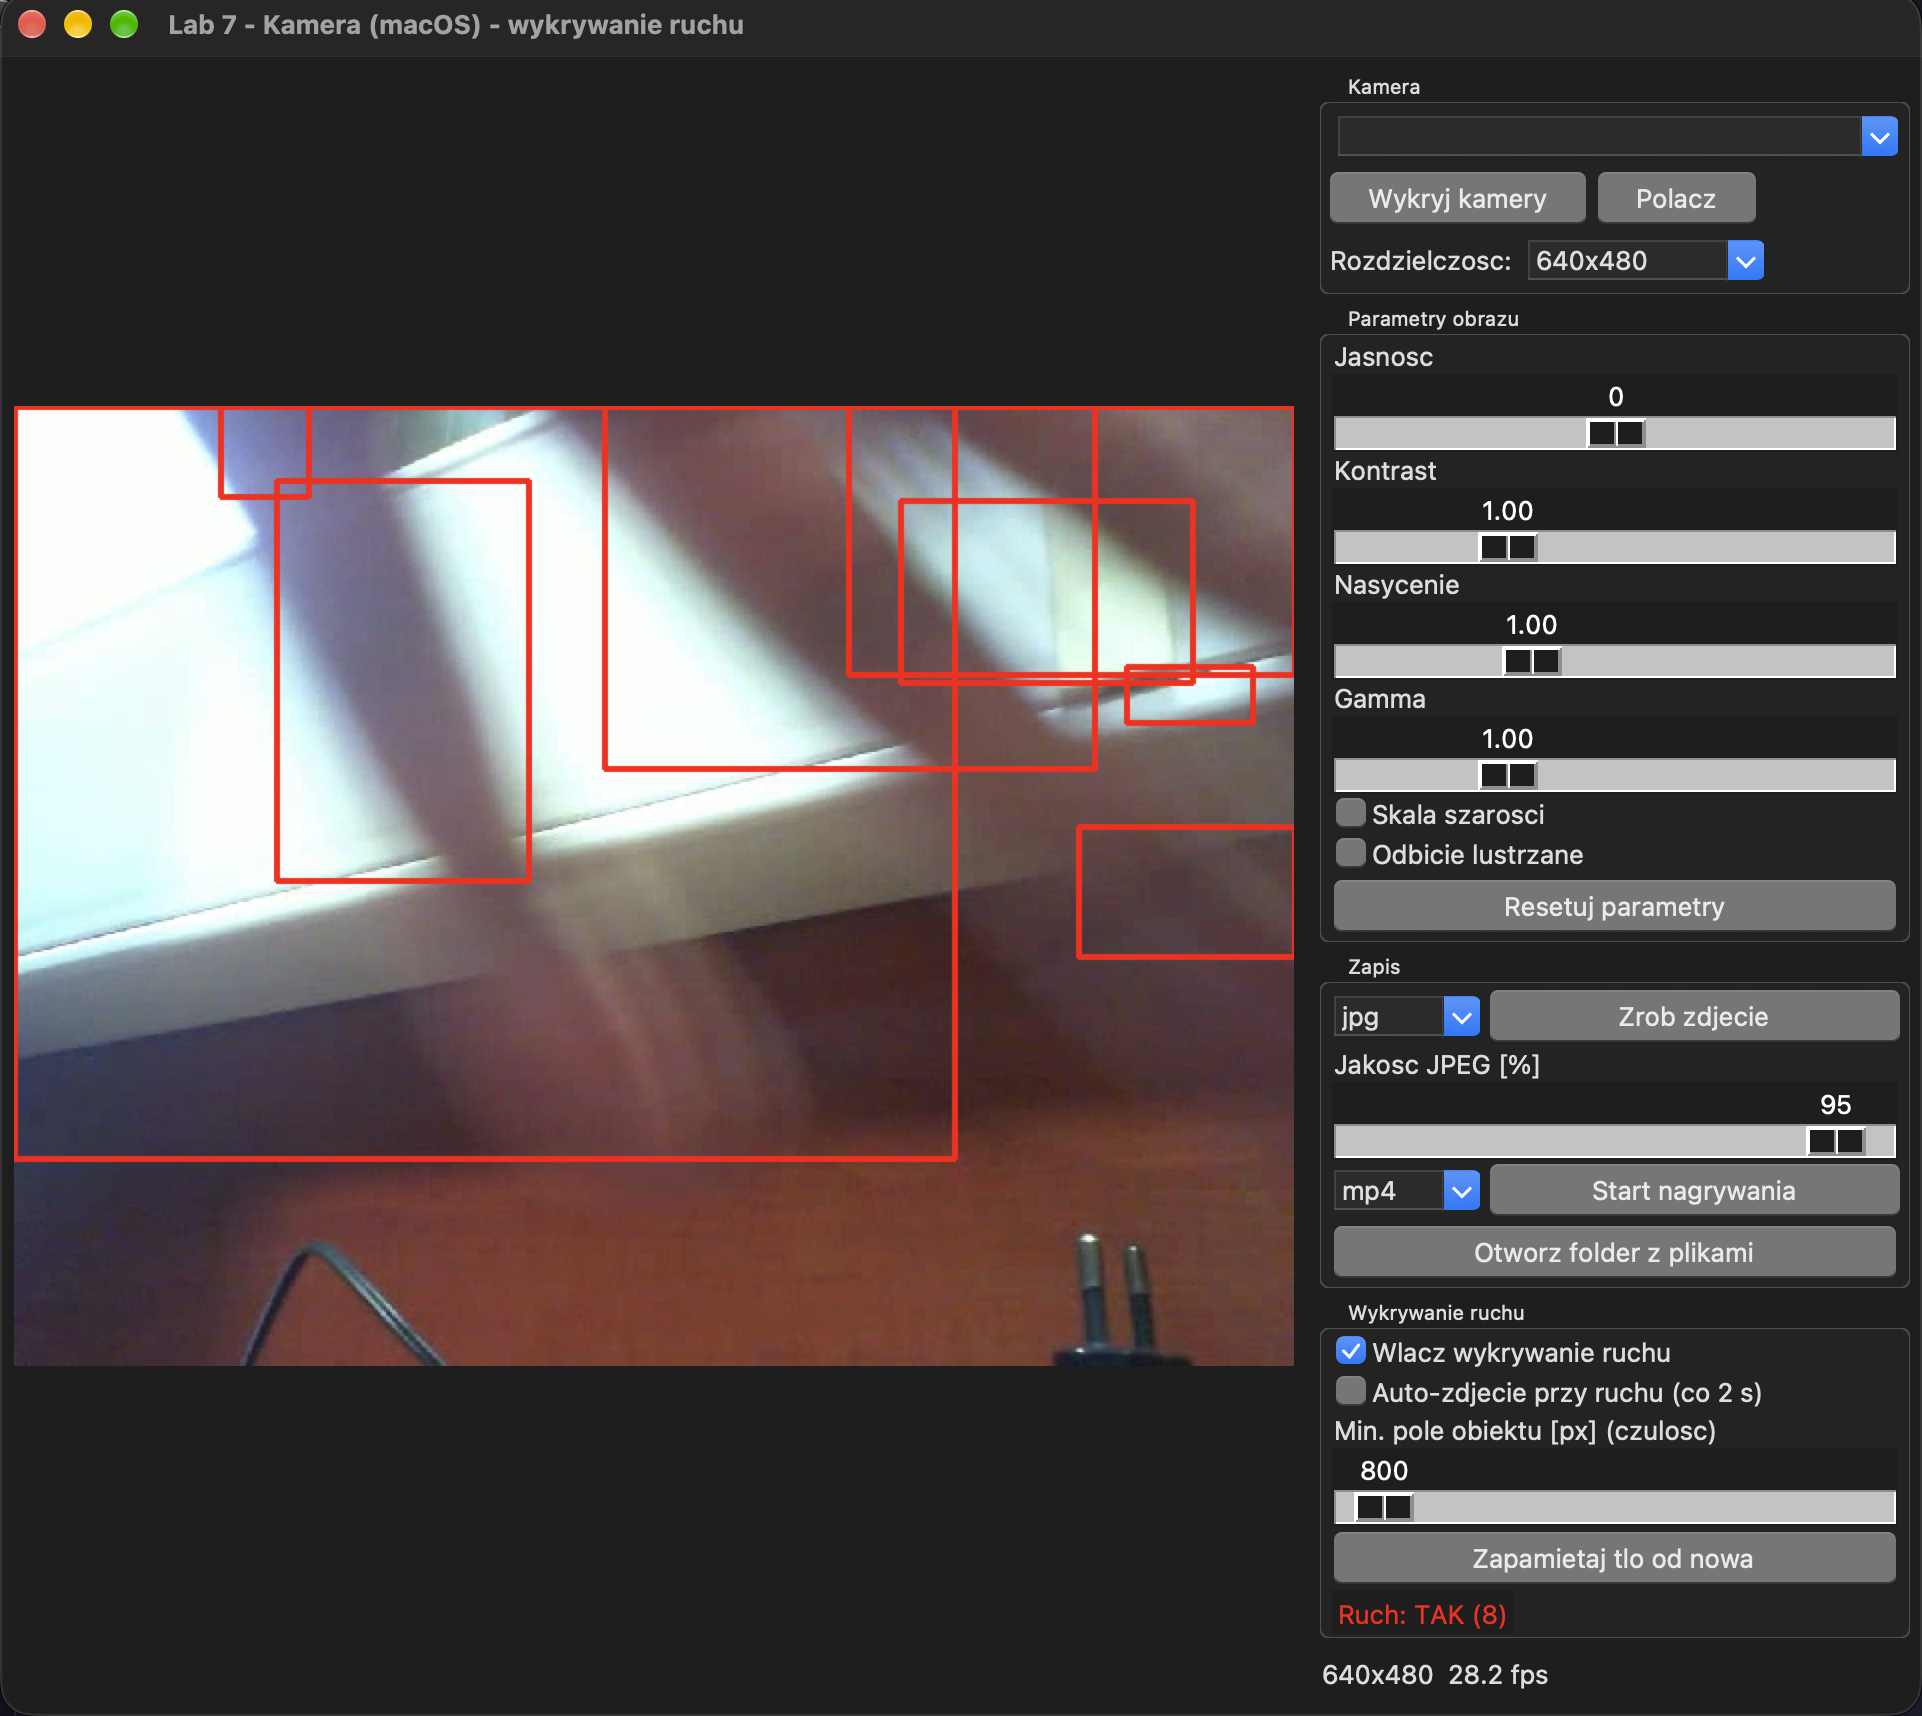
\includegraphics[width=0.85\textwidth]{ui_ruch.png}
  \caption{Okno programu \texttt{ruch\_mac.py} podczas wykrywania ruchu (źródłem obrazu jest nagranie
  z kamery USB2.0 Camera, $640\times480$)}
  \label{fig:okno}
\end{figure}

Program połączył się z kamerą LifeCam i nagrał film. Podczas nagrywania
zmieniano parametry obrazu. Nagrany plik \texttt{film\_20261123\_084552\_163.mp4} ma rozdzielczość
$1280\times800$, 292 klatki, 10,2 klatki na sekundę i czas trwania 28,5\,s. Otwiera się w
standardowych odtwarzaczach. Rysunek~\ref{fig:parametry} pokazuje klatki z tego filmu przy różnych
ustawieniach, a tabela~\ref{tab:parametry} średnią jasność (składowa V w przestrzeni HSV) i średnie
nasycenie (składowa S) tych klatek.

\begin{figure}[H]
  \centering
  \begin{subfigure}{0.32\textwidth}
\includegraphics[width=\linewidth]{klatka_oryginal.jpg}\caption{ustawienia domyślne}\end{subfigure}\hfill
  \begin{subfigure}{0.32\textwidth}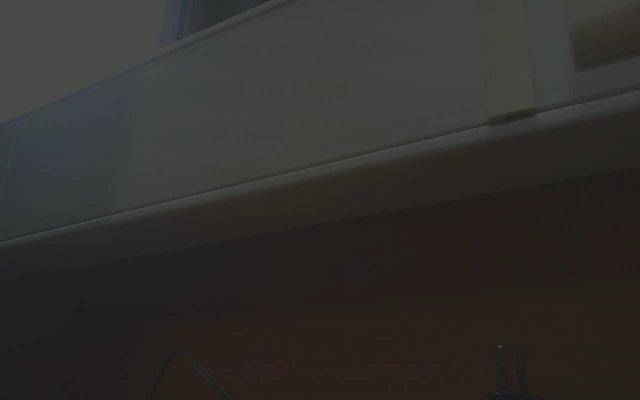
\includegraphics[width=\linewidth]{klatka_ciemno.jpg}\caption{obniżona jasność}\end{subfigure}\hfill
  \begin{subfigure}{0.32\textwidth}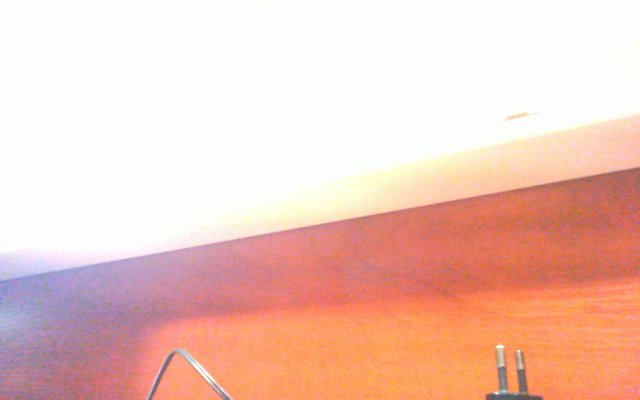
\includegraphics[width=\linewidth]{klatka_jasno.jpg}\caption{podwyższona jasność}\end{subfigure}\\[4pt]
  \begin{subfigure}{0.32\textwidth}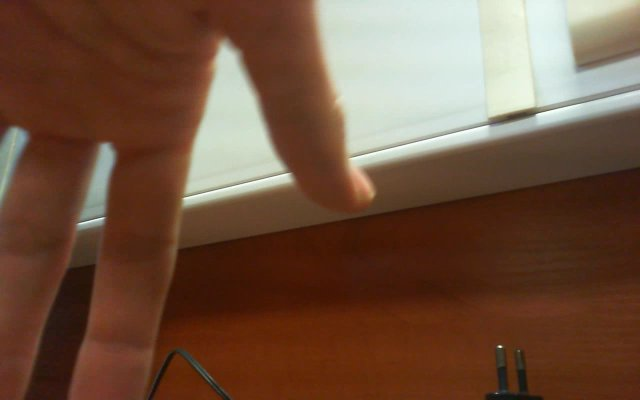
\includegraphics[width=\linewidth]{klatka_nasycenie.jpg}\caption{zwiększone nasycenie}\end{subfigure}\hspace{0.02\textwidth}
  \begin{subfigure}{0.32\textwidth}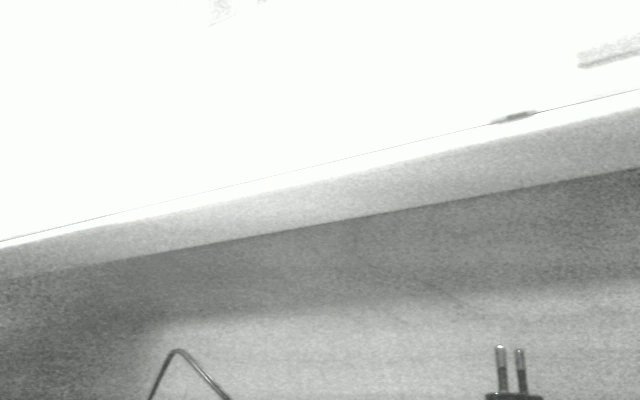
\includegraphics[width=\linewidth]{klatka_szarosc.jpg}\caption{skala szarości}\end{subfigure}
  \caption{Klatki z nagranego filmu przy różnych parametrach obrazu}
  \label{fig:parametry}
\end{figure}

\begin{table}[H]
  \centering
  \caption{Średnia jasność i nasycenie klatek z rysunku~\ref{fig:parametry} (skala 0–255)}
  \label{tab:parametry}
  \begin{tabular}{lcc}
    \toprule
    Ustawienie & Jasność V & Nasycenie S \\
    \midrule
    domyślne & 139 & 85 \\
    obniżona jasność & 51 & 40 \\
    podwyższona jasność & 241 & 62 \\
    zwiększone nasycenie & 115 & 148 \\
    skala szarości & 200 & 4 \\
    \bottomrule
  \end{tabular}
\end{table}

Wykrywanie ruchu (ocena wyższa) sprawdzono, poruszając ręką przed kamerą
(rys.~\ref{fig:ruch}). Ponieważ prostokąty nie są zapisywane do pliku, rysunek uzyskano,
przetwarzając nagrany film \texttt{film\_20261123\_084506\_652.mp4} ($640\times480$, 31 klatek na
sekundę) tą samą klasą \texttt{MotionDetector} z ustawieniami domyślnymi. Ruch wykryto w 140 z 584
klatek filmu.

\begin{figure}[H]
  \centering
  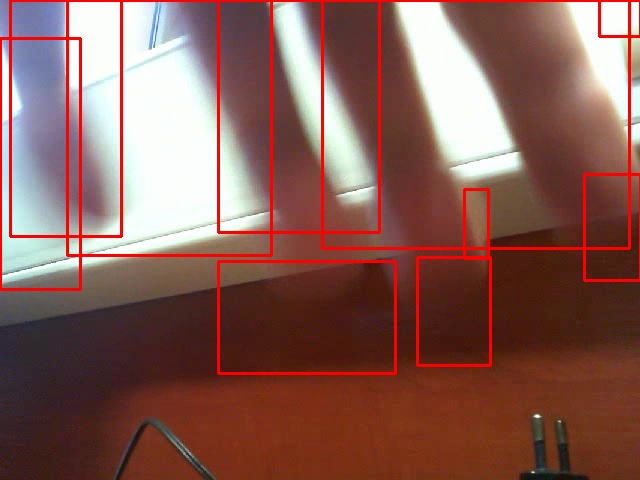
\includegraphics[width=0.6\textwidth]{ruch.jpg}
  \caption{Wykrywanie ruchu: poruszająca się ręka obrysowana czerwonymi prostokątami}
  \label{fig:ruch}
\end{figure}

\section{Wnioski}
Program realizuje polecenie prowadzącego: wykrywa podłączone kamery, pozwala wybrać kamerę i jej
rozdzielczość, zmienia nasycenie oraz jasność, kontrast i gamma, wykonuje zdjęcia (JPG, PNG, BMP)
i nagrywa filmy (MP4, AVI). Zmiany parametrów są widoczne w zapisanych plikach, co potwierdzają
pomiary w tabeli~\ref{tab:parametry}. W systemie macOS OpenCV nie zmienia trybu pracy kamery,
dlatego do odczytu nazw kamer i zmiany rozdzielczości potrzebne było AVFoundation; wszystkie
rozdzielczości z listy dały klatki o wybranym rozmiarze (tabela~\ref{tab:kamery}). Przy
rozdzielczości $1280\times800$ kamera LifeCam dawała tylko około 10 klatek na sekundę, a przy
$1280\times720$ około 30, prawdopodobnie z powodu ograniczonej przepustowości łącza USB 2.0 przy
klatkach nieskompresowanych. Na ocenę wyższą zrealizowano wykrywanie ruchu metodą odejmowania tła
(rysunek~\ref{fig:ruch}). Metoda działa w czasie rzeczywistym, ale reaguje na każdą zmianę obrazu,
także na zmianę oświetlenia lub parametrów obrazu, dlatego po takiej zmianie trzeba zapamiętać tło
od nowa.

\end{document}
